\documentclass[12pt]{article}
\usepackage[spanish]{babel}
\usepackage{float}
\usepackage[hidelinks]{hyperref}
\usepackage[utf8x]{inputenc}
\usepackage{hyperref}
\usepackage[style=listgroup,acronym,toc,hyperfirst,xindy]{glossaries}
\makeindex
\usepackage{graphicx}
\usepackage{wrapfig}
\graphicspath{{images/}}
\usepackage{parskip}
\usepackage{color}
\usepackage{listings}
\usepackage{subcaption}
\renewcommand{\lstlistingname}{Listado}
\usepackage{natbib}
\usepackage{url}
\usepackage{amsmath}
\makeglossaries
\usepackage[xindy]{imakeidx}
\usepackage{fancyhdr}
\usepackage{vmargin}
\usepackage{enumerate}
\usepackage[final]{pdfpages}

\lstset{
	basicstyle=\footnotesize,
	breakatwhitespace=false,         
	breaklines=true,                 
	captionpos=b,                    
	keepspaces=true,                
	numbers=left,                    
	numbersep=5pt,                  
	showspaces=false,                
	showstringspaces=false,
	showtabs=false,                  
	tabsize=4,
	frame=single
}

\lstset{language=Matlab,%
	%basicstyle=\color{red},
	breaklines=true,%
	morekeywords={matlab2tikz},
	keywordstyle=\color{blue},%
	morekeywords=[2]{1}, keywordstyle=[2]{\color{black}},
	identifierstyle=\color{black},%
	stringstyle=\color{lilas},
	commentstyle=\color{green},%
	showstringspaces=false,%without this there will be a symbol in the places where there is a space
	numbers=left,%
	numberstyle={\tiny \color{black}},% size of the numbers
	numbersep=9pt, % this defines how far the numbers are from the text
	emph=[1]{for,end,break},emphstyle=[1]\color{red}, %some words to emphasise
	%emph=[2]{word1,word2}, emphstyle=[2]{style},    
}

\usepackage{fancyhdr}
\usepackage{vmargin}
\setmarginsrb{3 cm}{2.5 cm}{3 cm}{2.5 cm}{1 cm}{1.5 cm}{1 cm}{1.5 cm}

\setglossarystyle{long}

% Acronym style
\newacronymstyle{ex-footnote}%
{%
	\GlsUseAcrEntryDispStyle{footnote}%
}%
{%
	\GlsUseAcrStyleDefs{footnote}%
	\renewcommand*{\genacrfullformat}[2]{%
		\firstacronymfont{\glsentryshort{##1}}##2%
		\expandafter\footnote\expandafter{\expandafter\glsentrylong\expandafter{##1}}%
	}%
	\renewcommand*{\Genacrfullformat}[2]{%
		\firstacronymfont{\Glsentryshort{##1}}##2%
		\expandafter\footnote\expandafter{\expandafter\glsentrylong\expandafter{##1}}%
	}%
	\renewcommand*{\genplacrfullformat}[2]{%
		\firstacronymfont{\glsentryshortpl{##1}}##2%
		\expandafter\footnote\expandafter{\expandafter\glsentrylongpl\expandafter{##1}}%
	}%
	\renewcommand*{\Genplacrfullformat}[2]{%
		\firstacronymfont{\Glsentryshortpl{##1}}##2%
		\expandafter\footnote\expandafter{\expandafter\glsentrylongpl\expandafter{##1}}%
	}%
}

\setacronymstyle{ex-footnote}



% Acronym list
\newacronym{oscar}{OSCAR}{Orbiting Satellite Carrying Amateur Radio}
\newacronym{satnogs}{SatNOGS}{Satellite Networked Operation Ground Stations}

% Title
\title{Estudio Previo Práctica 3}			
% Author
\author{Priscila Gómez Lizaga \\ Diego Cajal Orleans}								
% Date
\date{\today}										

\makeatletter
\let\thetitle\@title
\let\theauthor\@author
\let\thedate\@date
\makeatother

\pagestyle{fancy}
\fancyhf{}
\rhead{\theauthor}
\lhead{\thetitle}
\cfoot{\thepage}

\begin{document}

%%%%%%%%%%%%%%%%%%%%%%%%%%%%%%%%%%%%%%%%%%%%%%%%%%%%%%%%%%%%%%%%%%%%%%%%%%%%%%%%%%%%%%%%%

\begin{titlepage}
	\centering
    \vspace*{0.5 cm}
    
\includegraphics[scale = 0.75]{eina.png}\\[1.0 cm]	% University Logo
%    \textsc{\LARGE University of Cape Town}\\[2.0 cm]	% University Name
	\textsc{\Large 30357}\\[0.5 cm]				% Course Code
	\textsc{\large laboratorio de señal y comunicaciones}\\[0.5 cm]				% Course Name
	\rule{\linewidth}{0.2 mm} \\[0.4 cm]
	\setlength{\baselineskip}{2\baselineskip}
	{ \huge \bfseries \thetitle}\\
	\rule{\linewidth}{0.2 mm} \\[1.5 cm]
	
	\begin{minipage}{0.4\textwidth}
		\begin{flushleft} \large
			\emph{Autores:}\\
			\theauthor
			\end{flushleft}
			\end{minipage}~
			\begin{minipage}{0.4\textwidth}
			\begin{flushright} \large
			\emph{Nia:} \\
			684061 \\
			620622
												% Your Student Number
		\end{flushright}
	\end{minipage}\\[2 cm]
	
	{\large \thedate}\\[2 cm]
 
	\vfill
	
\end{titlepage}

%%%%%%%%%%%%%%%%%%%%%%%%%%%%%%%%%%%%%%%%%%%%%%%%%%%%%%%%%%%%%%%%%%%%%%%%%%%%%%%%%%%%%%%%%

%\tableofcontents
\pagebreak

%%%%%%%%%%%%%%%%%%%%%%%%%%%%%%%%%%%%%%%%%%%%%%%%%%%%%%%%%%%%%%%%%%%%%%%%%%%%%%%%%%%%%%%%%

\section{Determinación del género del locutor}
Se puede determinar el género del locutor sólo mediante segmentos sonoros. Los sonidos de vocales son cuasiperiódicos, por lo que se puede extraer una frecuencia fundamental (\textit{pitch}). Esta nos da la información de si el locutor es hombre o mujer, puesto que los hombres tienen por lo general frecuencias de pitch más bajas que las mujeres. Por el contrario, los sonidos sordos correspondientes a las consonantes no tienen una frecuencia fundamental producida por las excitaciones de las cuerdas vocales y por lo tanto no tienen información relevante acerca del locutor. Aunque puedan tener una frecuencia fundamental, esta tiene una naturaleza diferente, ya que este tipo de sonidos son producidos por una obstrucción en algún punto del tracto vocal.

Así, el primer segmento es válido para este objetivo, ya que corresponde a un sonido de vocal y se puede apreciar a simple vista la periodicidad. El segundo segmento no es válido por lo comentado anteriormente. Sin ningún procesado se aprecia que la forma de la onda de la segunda señal se asemeja más a ruido que a una señal periódica.

\section{Factor de ganancia}

\section{Autocorrelación de un tren de impulsos infinito}
La función de autocorrelación de un tren periódico de impulsos de duración infinita y periodo $T_0$ es una función rampa discreta infinita. Esta tiene valores nulos para todas las $n$ que no son múltiplos del periodo y un valor M para $n = M*T_0$, siendo M un número natural. Es nula para valores de $n$ negativos.

\begin{figure}[H]
	\centering
	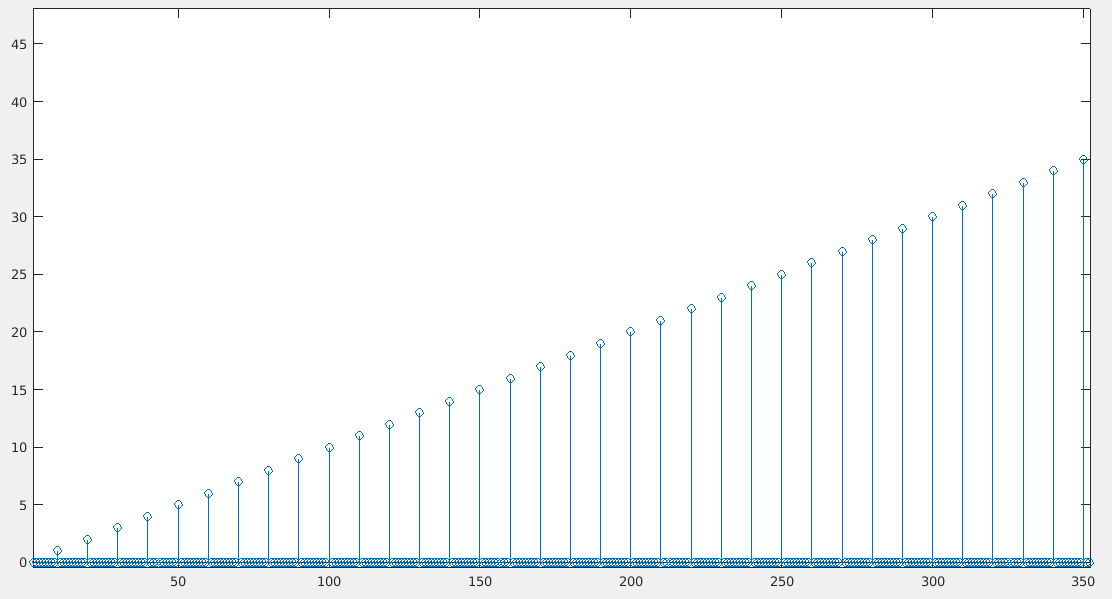
\includegraphics[width=0.7\textwidth]{autocorr_tren_infinito.png}
	\caption{Autocorrelación de un tren de impulsos infinito con $T_0 = 10$}
\end{figure}


\section{Autocorrelación de un segmento de N muestras}
La autocorrelación en el caso de un tren de N muestras es triangular. Es idéntica al caso infinito pero al llegar a la muestra N empieza a decrecer. Tiene por tanto 2N - 1 muestras. y es simétrica respecto a la muestra N.

\begin{figure}[H]
	\centering
	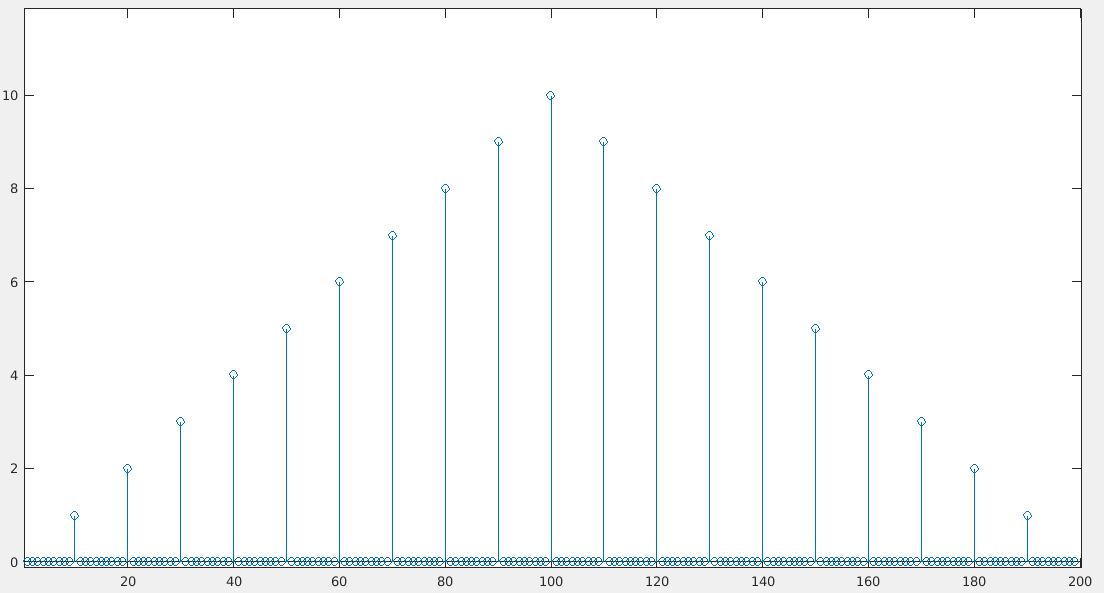
\includegraphics[width=0.7\textwidth]{autocorr_tren_finito.png}
	\caption{Autocorrelación de un tren de impulsos finito con $T_0 = 10$ y 100 muestras de duración}
	
\end{figure}


\section{Detección de pitch}

%\lstinputlisting[language=Matlab]{../Code/.m}

\end{document}
